\begin{center}
    {\LARGE \textbf{2012有机化学}} \\[2ex]
    {\large 时量180分钟 \quad 满分150分}
\end{center}

\vspace{0.5cm}
\noindent\textbf{注意事项:}
\begin{enumerate}[label=\arabic*., parsep=0pt, itemsep=0pt]
    \item 答题前,考生先将自己的姓名、学号、考场号、座位号填写在答题卡上,将条形码准确粘贴在考生信息条形码粘贴区。
    \item 考试结束后,将本试卷与答题纸一并收回。
    \item 回答各个问题时,将答案写在答题纸上,写在本试卷上无效。
\end{enumerate}

\vspace{0.5cm}
\noindent\textbf{一、完成反应(30 pts.)}

\begin{enumerate}[label=\arabic*., itemsep=3ex]
    \item 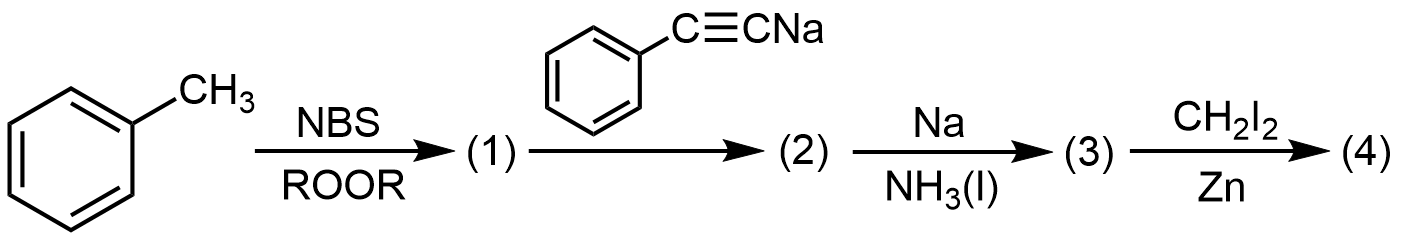
\includegraphics[scale=0.38, valign=c]{./Figure/2012/2012_1_1.png} 
    \item 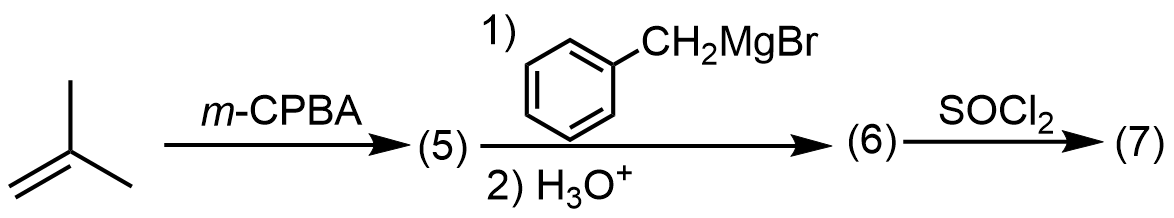
\includegraphics[scale=0.38, valign=c]{./Figure/2012/2012_1_2.png}
    \item 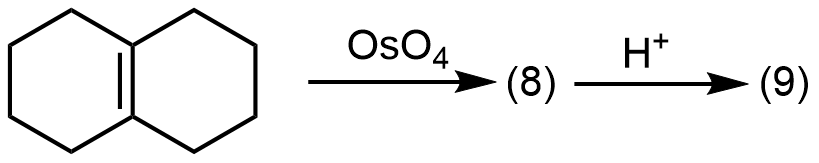
\includegraphics[scale=0.38, valign=c]{./Figure/2012/2012_1_3.png}
    \item 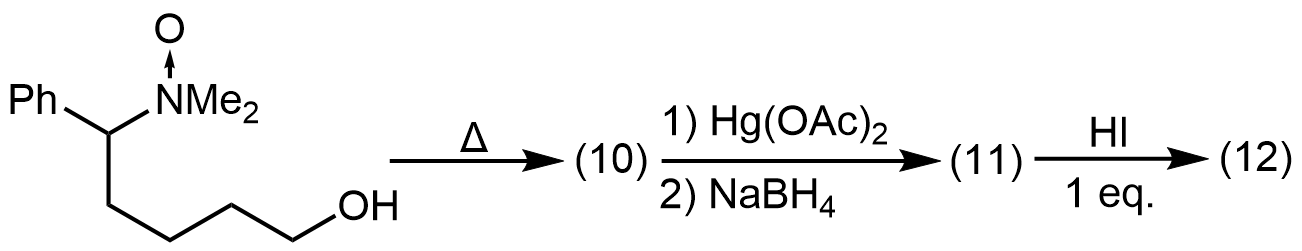
\includegraphics[scale=0.38, valign=c]{./Figure/2012/2012_1_4.png}
    \item 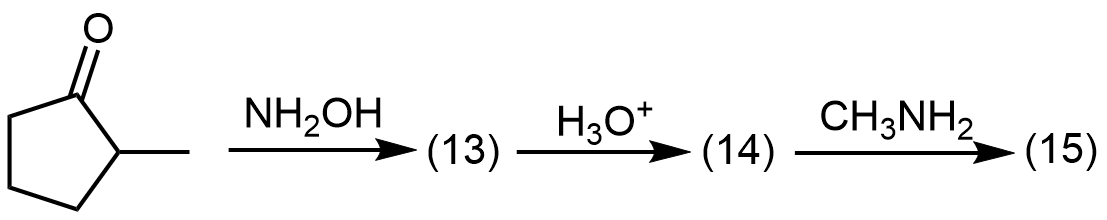
\includegraphics[scale=0.38, valign=c]{./Figure/2012/2012_1_5.png}
    \item 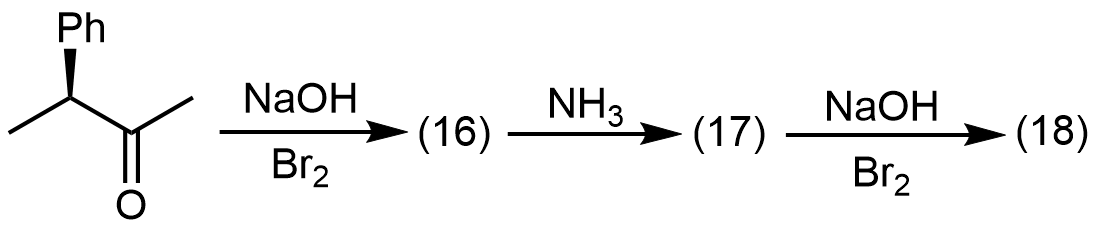
\includegraphics[scale=0.38, valign=c]{./Figure/2012/2012_1_6.png}
    \item 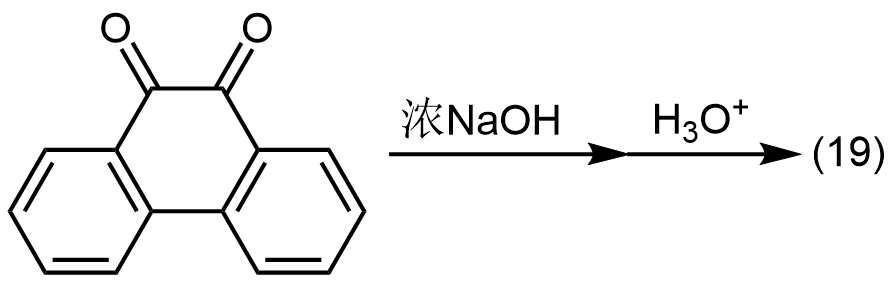
\includegraphics[scale=0.38, valign=c]{./Figure/2012/2012_1_7.png}
    \item 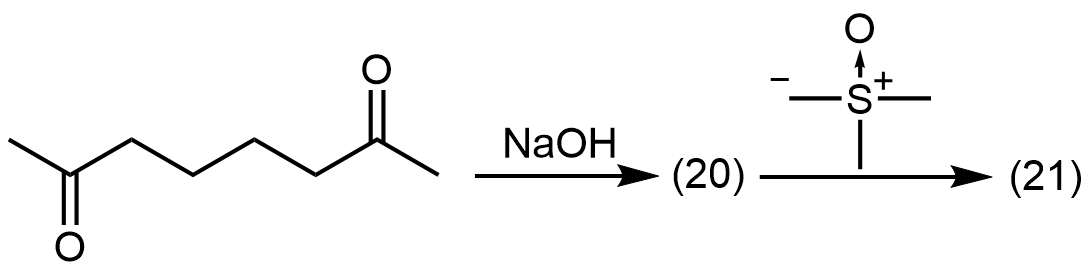
\includegraphics[scale=0.38, valign=c]{./Figure/2012/2012_1_8.png}
    \item 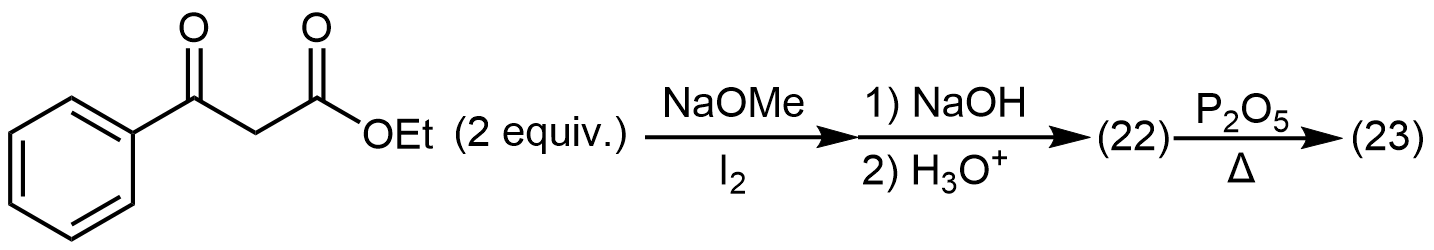
\includegraphics[scale=0.38, valign=c]{./Figure/2012/2012_1_9.png}
    \item 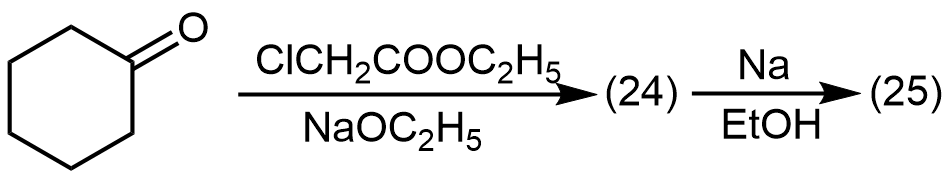
\includegraphics[scale=0.38, valign=c]{./Figure/2012/2012_1_10.png}

\end{enumerate}

\vspace{0.5cm}
\noindent\textbf{二、机理题(30 pts.)}

\begin{enumerate}[label=\arabic*., start=1, itemsep=1.5ex]
    \item 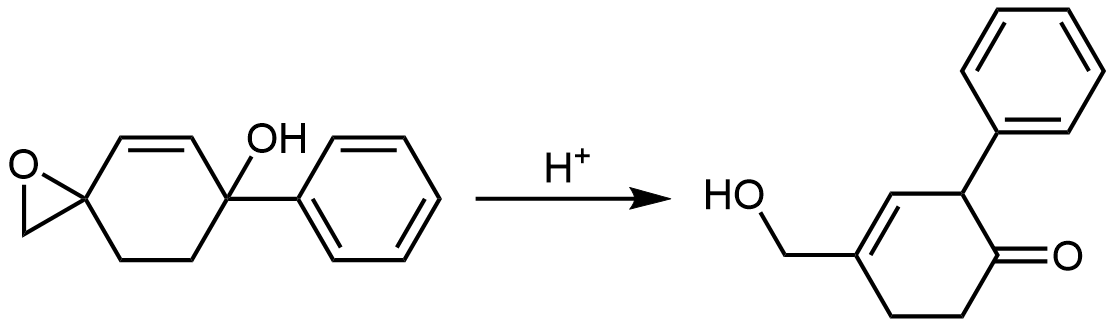
\includegraphics[scale=0.38, valign=c]{./Figure/2012/2012_2_1.png}
    \item 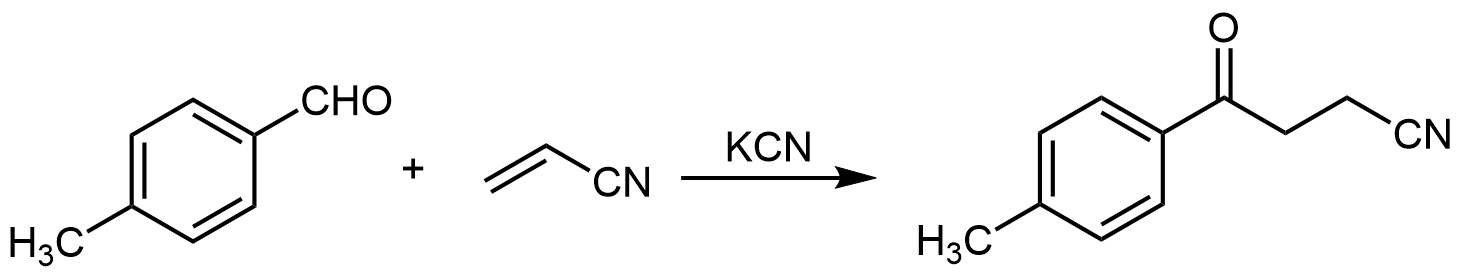
\includegraphics[scale=0.38, valign=c]{./Figure/2012/2012_2_2.png}
    \item 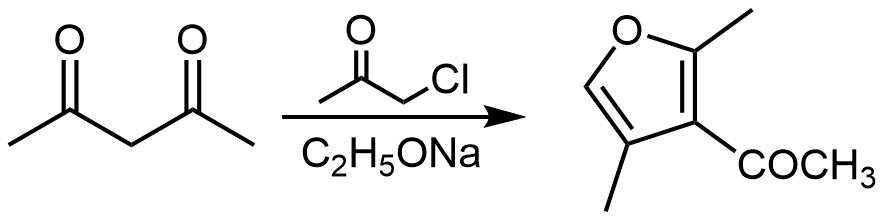
\includegraphics[scale=0.38, valign=c]{./Figure/2012/2012_2_3.png}
\end{enumerate}

\vspace{0.5cm}
\noindent\textbf{三、合成题(30 pts.)}

\begin{enumerate}[label=\arabic*., start=1, itemsep=1.5ex]

    \begin{figure}[htbp]
        \centering
        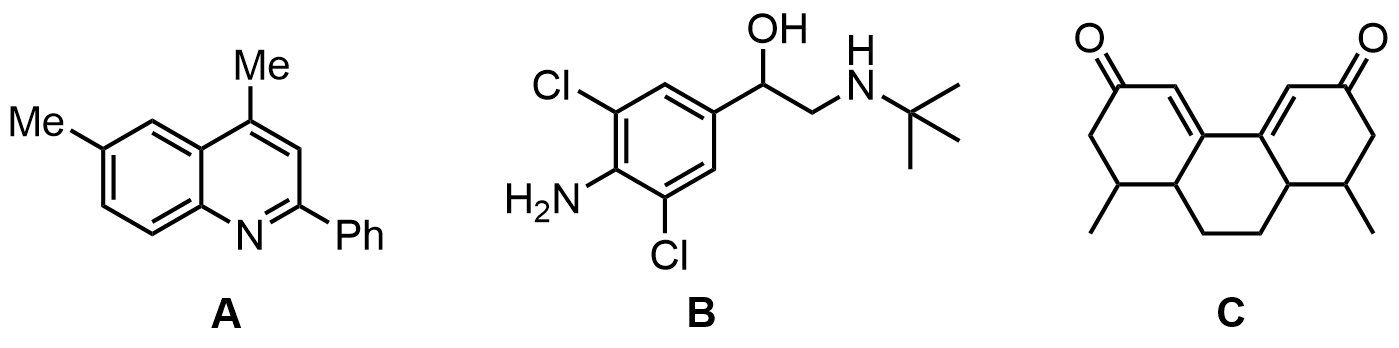
\includegraphics[scale=0.38]{./Figure/2012/2012_3.png}
    \end{figure}
    \item 以苯及小于等于3个碳的有机物为原料及必要的无机试剂合成\textbf{A}
    \item 以丙酮为唯一有机原料合成叔丁胺，再以叔丁胺、苯胺及小于等于2个碳的有机物为原料及必要的无机试剂合成瘦肉精\textbf{B}
    \item 以小于等于2个碳的有机物为原料合成\textbf{C}
\end{enumerate}

\vspace{0.5cm}
\noindent\textbf{四、综合题(20 pts.)}

\begin{figure}[htbp]
    \centering
    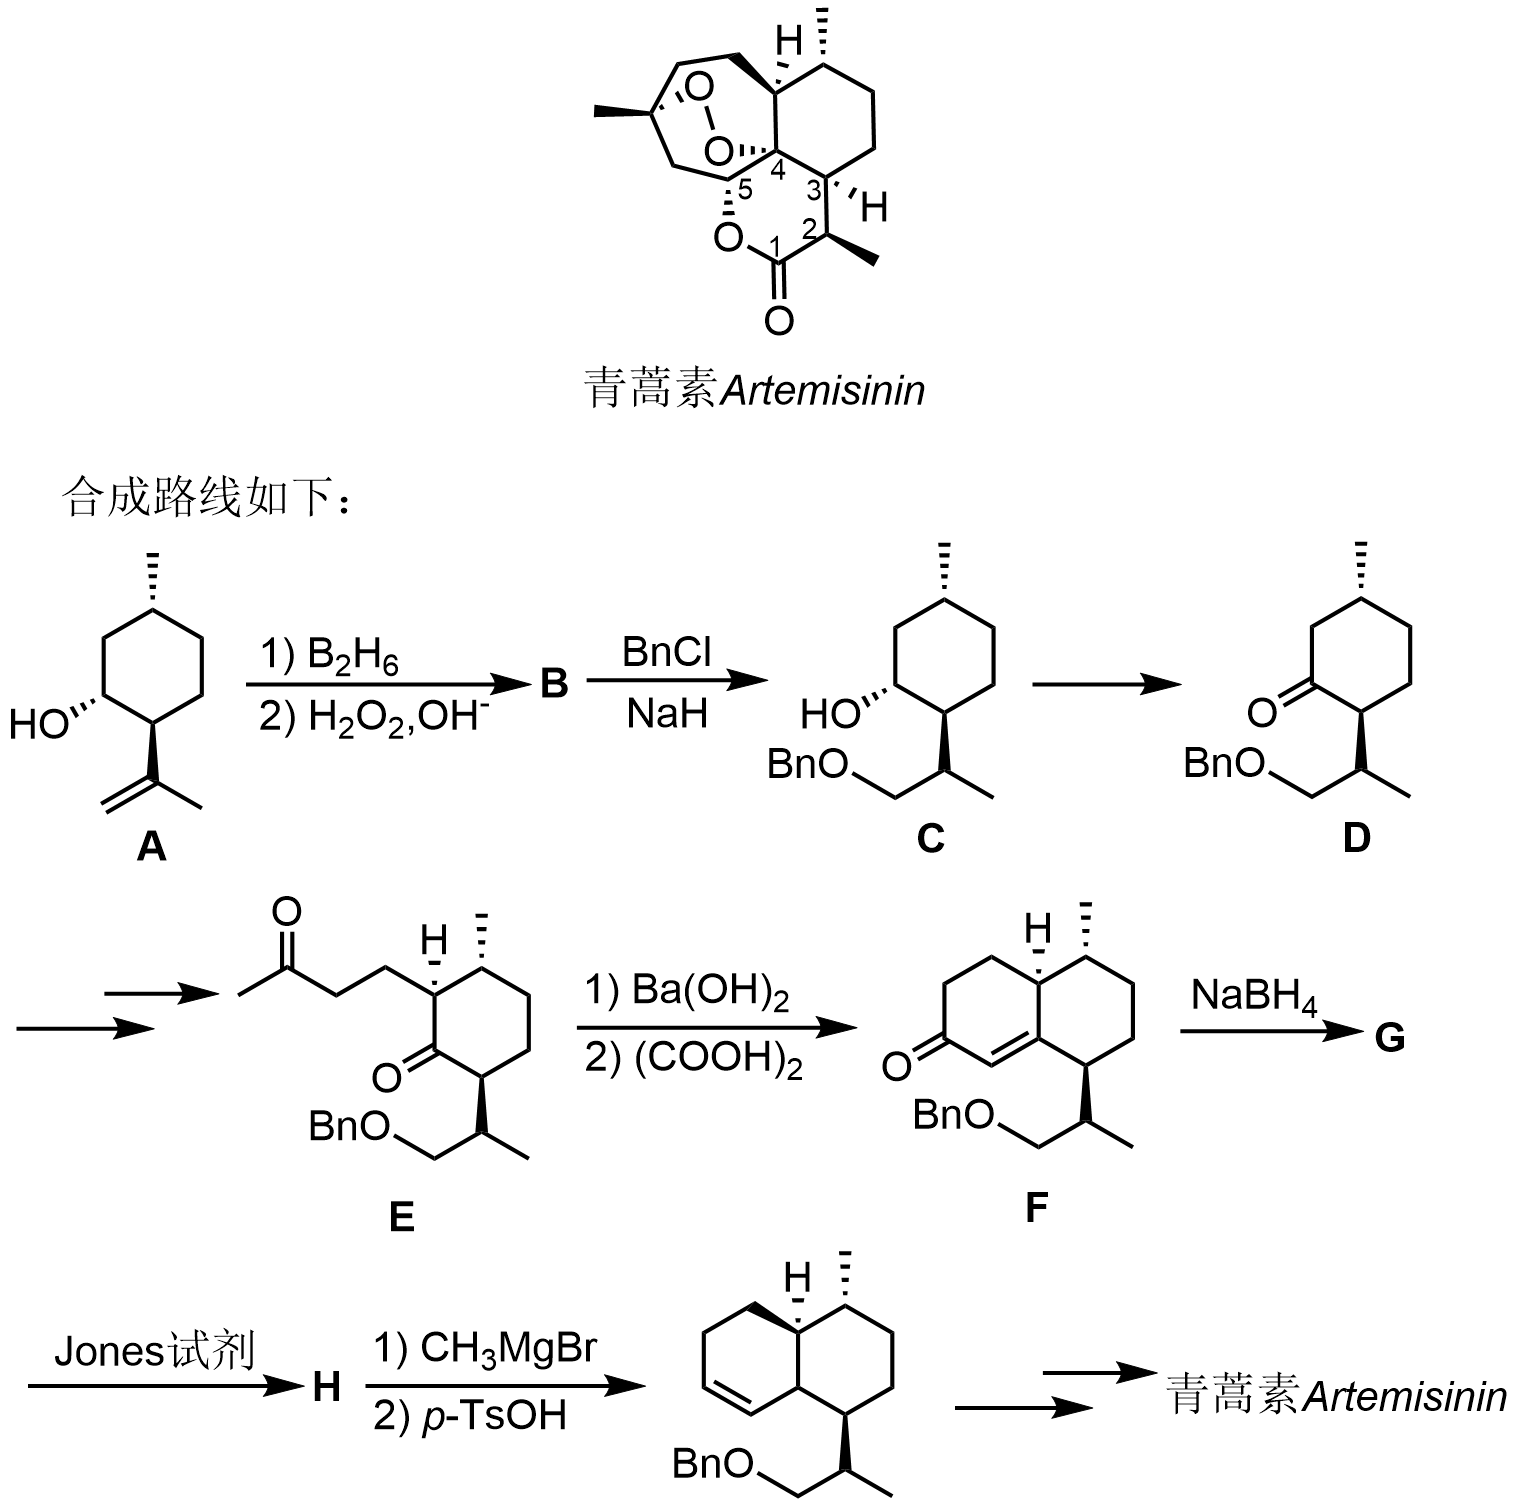
\includegraphics[scale=0.37]{./Figure/2012/2012_4.png}
\end{figure}

\begin{enumerate}[label=\arabic*., itemsep=1.2ex]
    \item 青蒿素分子中有几个手性碳原子？写出内酯环上C-2、C-3、C-4、C-5的构型。(6 pts.)
    \item 画出中间体B、G、H的结构式。(6 pts.)
    \item 请写出合成路线中从C到D所需的反应条件。(2 pts.)
    \item 写出从E到F的反应机理。(6 pts.)
\end{enumerate}

\vspace{0.5cm}
\noindent\textbf{五、实验题 略}